%%=============================================================================
%% Elastic stack
%%=============================================================================

\chapter{Elastic stack}
\label{ch:elasticstack}

Hier zal getracht worden aan de hand van \ref{fig:elasticstackoverview} de werking van Elastic stack uit te leggen. Dit zal nog heel oppervlakkig gebeuren maar zou het mogelijk moeten maken een beter inzicht te creëren in de komende hoofdstukken.

\begin{figure}[h]
	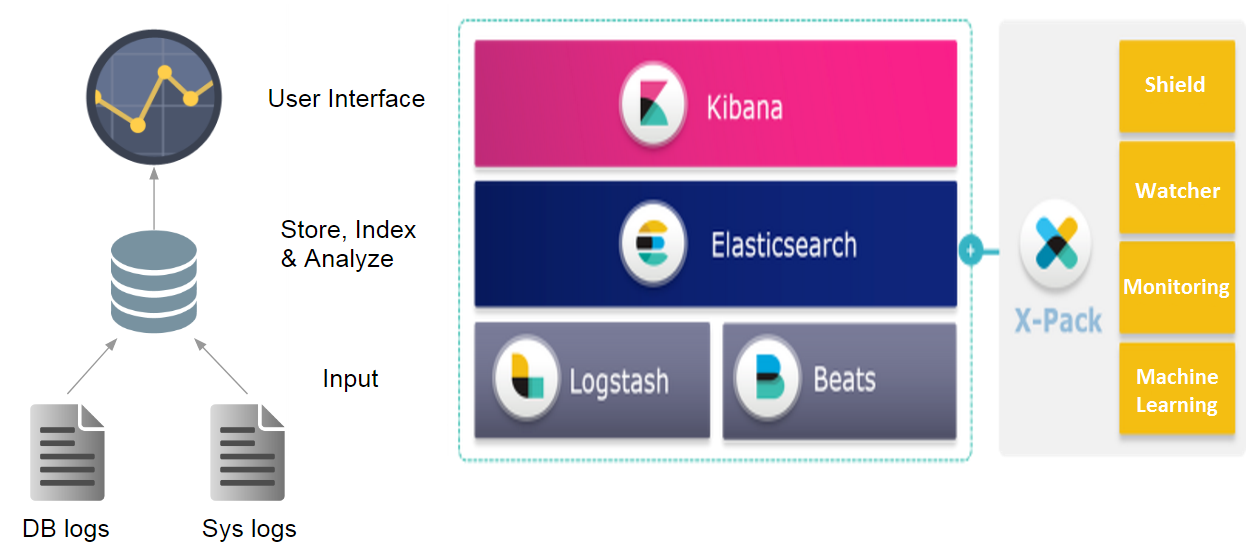
\includegraphics[width=16cm]{img/elasticstackoverview}
	\caption{Overzicht Elastic stack}
	\label{fig:elasticstackoverview}
\end{figure}

Zoals te zien is op in \ref{fig:elasticstackoverview} bestaat Elastic stack uit drie niveaus. 
Om de werking uit te leggen moet onderaan begonnen worden. Op dit niveau staan Logstash en Beats. 
Beats staat in voor het verzamelen van alle log files. Het is een tool die alle logs kan verzenden naar een centrale server waarop Logstash zich dan bevind. Logstash leest log files en verwerkt alle nieuwe lijnen die in de file geschreven worden. Het neemt lijn per lijn en verwerkt deze tot een json element.

Een niveau hoger is Elasticsearch te vinden. Elasticsearch staat in voor het opslaan en verwerken van alle input dat het krijgt van Logstash. Het krijgt de json elementen die logstash aanmaakt en slaat deze zo op in zijn databank. Doordat het json elementen zijn werkt de manier van zoeken op een andere dan met sql-opdrachten. In het verder verloop van deze bachelorproef zal gesproken over elementen dit zijn dan json elementen die zich in de database bevinden.

Kibana is de grafische kant van het hele gebeuren. Hier kan een overzicht van alle elementen getoond worden, het uitvoeren van Elasticsearch queries, het maken van grafieken, \dots.
Eenmaal alles geïmplementeerd is zal (in normale omstandigheden) alle acties via Kibana verlopen.

Helemaal rechts kan dan nog X-Pack gevonden worden. Dit is een samen raapsel van tools die werken met Elastic stack. 